%!TEX program = xelatex
\documentclass[conference]{IEEEtran}
\IEEEoverridecommandlockouts
% The preceding line is only needed to identify funding in the first footnote. If that is unneeded, please comment it out.
\usepackage{cite}
\usepackage{bm}
\usepackage{amsmath,amssymb,amsfonts}
\usepackage{algorithmic}
\usepackage{graphicx}
\usepackage{textcomp}
\usepackage{listings}
\usepackage{fontspec} % 定制字体
\newfontfamily\menlo{agave Nerd Font}
\usepackage{xcolor}

\def\BibTeX{{\rm B\kern-.05em{\sc i\kern-.025em b}\kern-.08em
    T\kern-.1667em\lower.7ex\hbox{E}\kern-.125emX}}
\begin{document}

\title{Dynamic I/O Model Recommendation System With Machine Learning\\
{\footnotesize \textsuperscript{*}Note: Sub-titles are not captured in Xplore and
should not be used}
\thanks{Identify applicable funding agency here. If none, delete this.}
}

\author{\IEEEauthorblockN{1\textsuperscript{st} Given Name Surname}
	\IEEEauthorblockA{\textit{dept. name of organization (of Aff.)} \\
		\textit{name of organization (of Aff.)}\\
		City, Country \\
		email address or ORCID}
	\and
	\IEEEauthorblockN{2\textsuperscript{nd} Given Name Surname}
	\IEEEauthorblockA{\textit{dept. name of organization (of Aff.)} \\
		\textit{name of organization (of Aff.)}\\
		City, Country \\
		email address or ORCID}
}

\maketitle

\begin{abstract}
	In a typical database and file system, using asynchronous I/O is generally a good way to optimize processing efficiency.
	However, each process and application mainly focus on its own performance, rarely consider the global performance of the system.
	In this work, in order to balance the I/O performance and resources in a system, we use Machine Learning(ML) techniques to learn I/O model's performance,
	and set up a client/server system based on gRPC to recommend the more efficient I/O model under different system loads. Which is high performance, scalable, cross-platform and easy to adapt.
	The experimental result shows that our system has a 15\% performance improvement compared to using asynchronous I/O alone and only cost little system resources.

\end{abstract}

\renewcommand\IEEEkeywordsname{Keywords}
\begin{IEEEkeywords}
	asynchronous I/O, synchronous I/O, Machine Learning, performance prediction, gRPC
\end{IEEEkeywords}

\section{Introduction}

% \begin{itemize}
%     \item Data center is popular and I/O is one of the bottlenecks
%     \item asynchronous and synchronous I/O
%     \item Machine Learning
%     \item structure of my system
% \end{itemize}

With revolution of “Big Data” and “Cloud Computing”, data center has expended to a large scale and data has grown exponentially.
Therefore, data center has to process hundreds of millions of pictures and hundreds of billions of messages each day.
How to improve processing efficiency is a hot issue of a data center.
Due to the huge speed gap between CPU and I/O device, I/O is one of the bottlenecks of the issue.
Using asynchronous I/O is a common way to boost I/O speed. Synchronous and asynchronous I/O are two types of I/O synchronizations as  \emph{\textbf{\large{figure 1}}} shows.
In a synchronous I/O job, it starts a thread for I/O operation, and it would hang immediately until the operation is finished.
While in an asynchronous I/O job, it would start a thread to send a I/O request to Kernel by calling a function, if the request is accepted successfully, it continues to process other jobs.
The kernel signals the calling thread when the operation is finished, then the thread interrupts its current job and processes the data from the I/O operation as soon as possible.
However, using asynchronous I/O frequently requires much CPU resources and the I/O's latency would become higher when the I/O's depth is longer.

\begin{figure}[htbp]
	\centering
	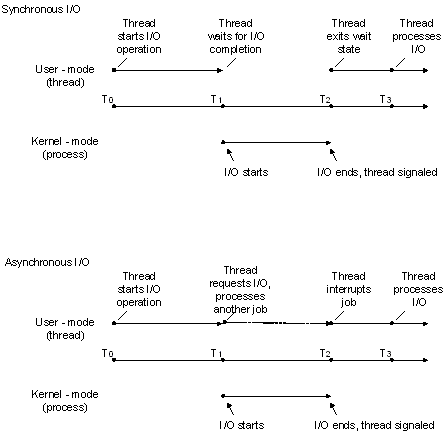
\includegraphics[width=0.45\textwidth]{fig2bedit.png}
	\caption{Asynchronous and Synchronous I/O}
	% \label{fig}
\end{figure}

To help improve system I/O and processing efficiency, we purpose to combine I/O with Machine Learning(ML). The I/O synchronizations of each I/O's engine
have different performance when it is facing different kinds of I/O job and different system load. Collecting these I/O data and training into a Decision Tree model
which can predict the most suitable I/O method in current situation. And setting up a Client/Server-based recommendation system using gRPC framework to decide using which kind of I/O for each I/O job.


The main challenge of our system is performance, since each I/O job have to call the server for the better I/O method which cost much time on process communication and prediction.
To solve the related problems, we use memory cache and gRPC framework. The data is serialized to protocol buffers and passed by stream, meanwhile, store the hot data into cache.
Therefore, the communication's time will be shortened and reuse the prediction result. After the improvements applied in our system, Running the same task has an efficiency increase of nearly 15\%.

In summary, we have made the following contributions in our paper:
\begin{enumerate}
	\item Train a Decision Tree model which can predict the best I/O method base on the current system load.
	\item We build a Client/Server-based, lightweight and scalable system using gRPC to help each I/O job improve efficiency.
	\item Run a script to make the system self-optimization daily.
\end{enumerate}

The rest of the paper is organized In Sect. 2 we show the design
of recommendation system and propose its implementation in Sect. 3. In Sect. 4 we introduce
the experiment configuration and result. The related work is discussed in Sect.
5. Finally, we conclude the paper and talk about the future work in Sect. 6.



\section{Design}
In this section we talk about the goals of our system first and then show the overview architecture.

\subsection{Goals}
According to the motivation of this paper, we should obtain the following goals
on system design:
\begin{itemize}
	\item High-Performance. Our system should calculate the prediction in a short time and return it to the client on time, otherwise it would become a burden.
	\item Cross-Platform. The system should have the ability to support variable of programming language, because the clients are written in different language.
	\item Scalable. The system should be easy to add feature to afford different scenarios.
	\item Self-Optimization. The system should have the ability to optimize itself daily for hot data.
\end{itemize}

\subsection{Overview}
Figure 2 show the architecture of the recommendation system. The system is built based on gRPC
to archive the goals of High-Performance, Cross-Platform and Scalable. The redis is deployed to store the hot query data.

\begin{figure}[htbp]
	\centering
	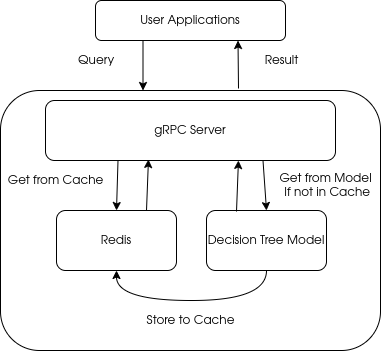
\includegraphics[width=0.4\textwidth]{architecture.png}
	\caption{Architecture}
	% \label{fig}
\end{figure}

A detail procedure of user applications get the predictions from the system is described as follow by referring Fig.2
\begin{enumerate}
	\item Application prepares the characteristic parameters for the I/O jobs.
	\item Remote call predict method through gRPC, waiting for the result or continue to other jobs if using asynchronous call.
	\item The method would first check the query if it's in cache, if in, return it to the application first and update it in cache.
	\item If it is not in cache, pass the parameters into Decision Tree model to predict the result. Then, return the result, and store it into cache.
	\item Check the hottest queries in a day, collect them as the training data set to update the Decision Tree model.
\end{enumerate}


\subsection{Techniques}

\begin{itemize}

	\item \emph{Fio}

	      Fio was written by Jens Axboe <axboe@kernel.dk> to enable flexible testing of
	      the Linux I/O subsystem and schedulers. We use fio to simulate different I/O jobs in actual production environment, which we can chang it I/O engine, I/O depth, file size and so on.

	\item \emph{Machine Learning}

	      Machine Learning is a method of data analysis that automates analytical model building.
	      It is a branch of artificial intelligence based on the idea that systems can learn from data, identify patterns and make decisions with minimal human intervention.
	      It is very useful to predict the best I/O method in our system.
	      % "https://www.sas.com/en_us/insights/analytics/machine-learning.html"

	\item \emph{Decision Tree}

	      A decision tree is a decision support tool that uses a tree-like model of decisions and their possible consequences, including chance event outcomes, resource costs, and utility. It is one way to display an algorithm that only contains conditional control statements.
	      Decision trees are commonly used in operations research, specifically in decision analysis, to help identify a strategy most likely to reach a goal, but are also a popular tool in machine learning.
	      It is easy to understand and implement, and can make feasible and effective results for large data sources in a relatively short time. At the same time, it is highly efficient. The decision tree only needs to be constructed once and used repeatedly,
	      and the maximum number of calculations for each prediction does not exceed the depth of the decision tree. By using Decision Tree can archive the goal of High-Performance.
	      % "https://en.wikipedia.org/wiki/Decision_tree"

	\item \emph{gRPC framework}

	      To archive the goals of High-Performance, Cross-Platform and Scalable, using gRPC framework is one of the best choice.
	      gRPC is a modern open source high performance RPC framework that can run in any environment. It can efficiently connect services in
	      and across data centers with pluggable support for load balancing, tracing, health checking and authentication.
	      It is also applicable in last mile of distributed computing to connect devices, mobile applications and browsers to backend services.
	      UDP socket may higher transmission speed, but it is hard apply features and may lose the data.

	      % https://grpc.io/
	\item \emph{Atomic}

	      To speed up the system, we use atomic variables instead of locks, which have better performance in high concurrency scenarios compare to locks.
	      It is very easy to deploy the redis to archive High-Performance.

	\item \emph{Redis}

	      Redis is an in-memory data structure store, which is usually used as cache.
\end{itemize}

\subsection{Discussion}
\begin{itemize}
	\item How to improve the performance?

	      First, gRPC is a High-Performance and lightweight framework especially in intranet environment.

	\item How to Optimize itself?

	      While running the system, a script will run daily to look for the data in redis, to check if there is any hot data that has called for most time.
	      That is one of the most import data for this environment. Then, collect it as the training data set, and re-train the model again.
	      By doing this, the system has been updated without taking it offline, just like hot repair.

\end{itemize}


\section{Implementation}
We implement all above improvements on a Linux system, which is similar to the data center environment, and the disk we use is a West Data 256G SSD.
\begin{itemize}

	\item We used Fio and cpulimit tool to test the I/O performance of different I/O methods in our system,
	 we can change different parameters to simulate single task or multitasking and random read or random write.
	 And we mainly collect 4K random read/write performance of the system, one of the most important indicators is iops(I/O per second).
	 After collecting the data, we preprocess it. We use one-hot encoding to convert the string into a vector form, and select the data with the highest iops as our training data.


	      \begin{lstlisting}[language={bash},
		basicstyle=\normalsize\menlo,
        numbers=left]
; -- start job file --
[global] ; global parameters
rw=randread 
bs=4k
direct=1
[job1]
filename=./mytest
iodepth=4
ioengine=io_uring
size=1G
numjobs=1
\end{lstlisting}

	\item After preprocessing the data, we combine the ioengine and iodepth as the classification label, then import the data into Decision Tree Model. 
	We save the trained model as a pickle file, so we don't need to train it every time we use it, besides, we can deploy it in similar environment.
	\item After the model is ready, we build a gRPC server and load the model to memory waiting for clients' calls.
\end{itemize}


\section{Evaluation}
	In this section, we evaluate our recommendation system by comparing it performance in different situations with only using synchronous or asynchronous I/O.
	And we have prepared 20 I/O task for the evaluation.
\begin{itemize}

	\item We used Fio and cpulimit tool to test the I/O performance of different I/O methods in our system,
	 we can change different parameters to simulate single task or multitasking and random read or random write.
	 And we mainly collect 4K random read/write performance of the system, one of the most important indicators is iops(I/O per second).
	 After collecting the data, we preprocess it. We use one-hot encoding to convert the string into a vector form, and select the data with the highest iops as our training data.


	      \begin{lstlisting}[language={C},
		basicstyle=\normalsize\menlo,
        numbers=left]
const std::vector<std::vector<std::string>> jobs = {
//size(KB)  rw
{"31174", "read"},      
{"96871", "write"},      
{"94486", "randread"},
{"40694", "randwrite"}, 
{"46993", "read"},       
{"76150", "write"},
{"76967", "randread"},  
{"128517", "read"},      
{"473399", "write"},
{"338556", "randread"}, 
{"130019", "randwrite"}, 
{"334198", "write"},
{"31174", "randread"},  
{"96871", "randwrite"},  
{"94486", "read"},
{"46993", "randread"},  
{"2309", "randwrite"},   
{"76150", "read"},
{"76967", "write"},     
{"323408", "randread"},  
{"128517", "randwrite"}
};
\end{lstlisting}

	\item compare single I/O work performance between used and none-used our system
\begin{figure}[htbp]
	\centering
	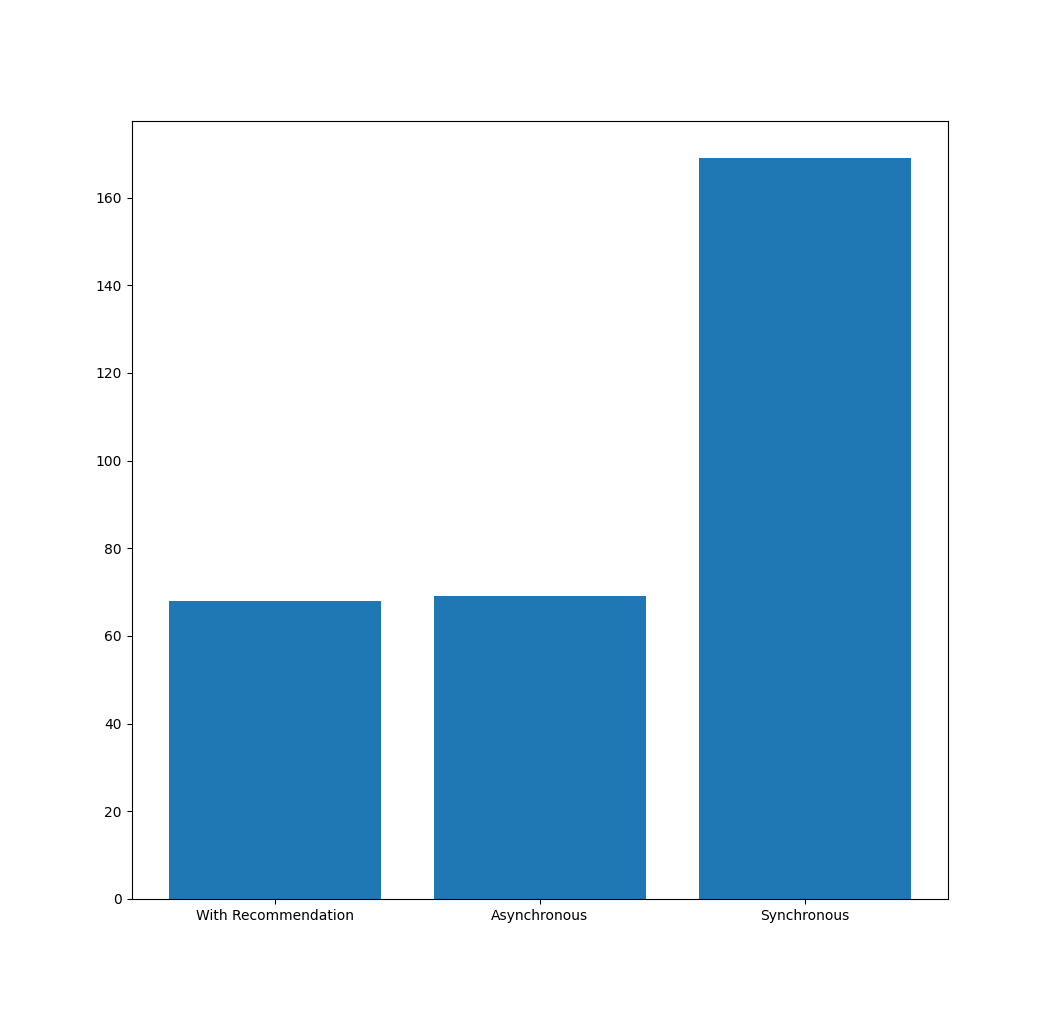
\includegraphics[width=0.4\textwidth]{Figure_2.png}
	\caption{Single Task}
	% \label{fig}
\end{figure}
	\item compare multi I/O works performance between used and none-used our system
\begin{figure}[htbp]
	\centering
	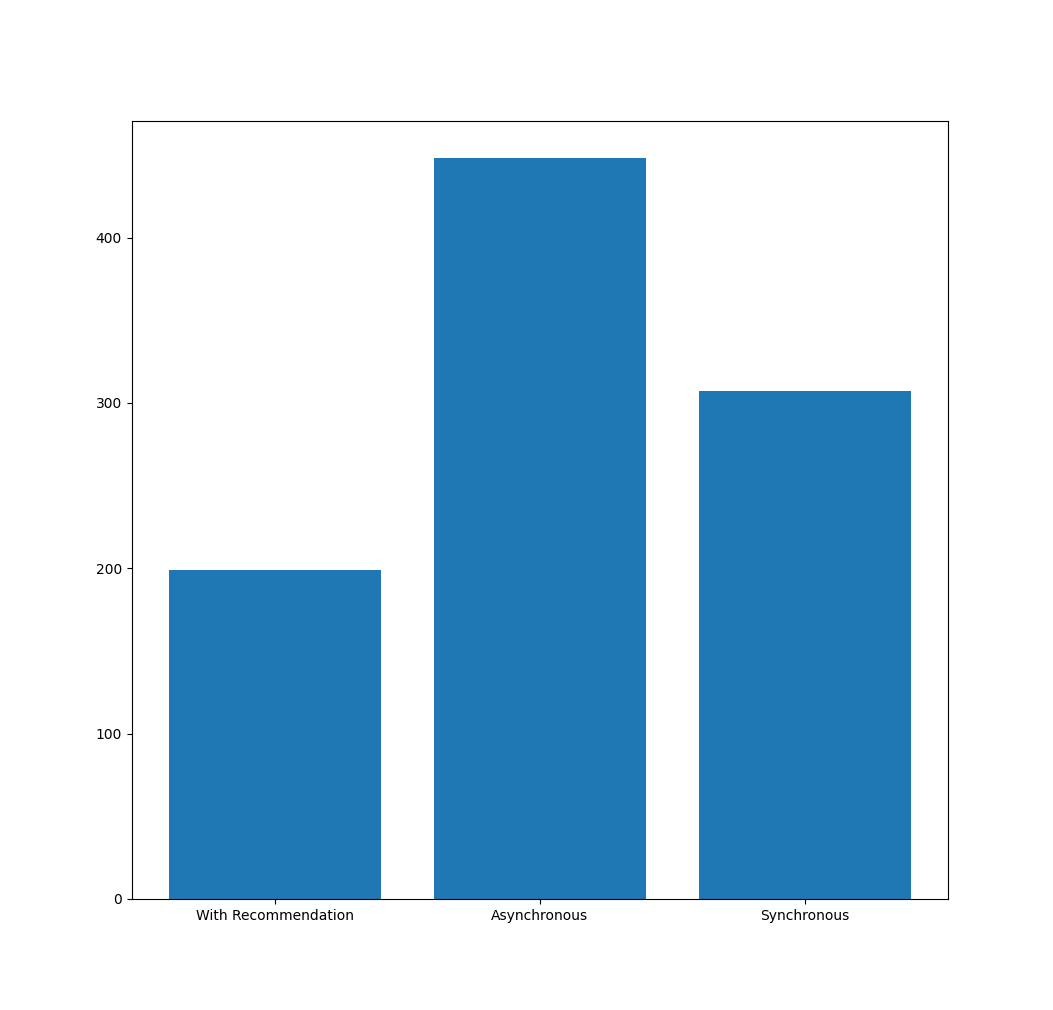
\includegraphics[width=0.4\textwidth]{Figure_1.png}
	\caption{Multitasking}
	% \label{fig}
\end{figure}
	\item io-uring performance
	\item evaluate the cost of gRPC
	\item evaluate the cost of Decision Tree
\end{itemize}

\section{Related Work}
\begin{itemize}
	\item hot issue in I/O
\end{itemize}

\section{Conclusion}
improvement of our system and future usage scenario

\section*{Acknowledgment}


% \section*{References}


\begin{thebibliography}{00}
	\bibitem{b1} G. Eason, B. Noble, and I. N. Sneddon, ``On certain integrals of Lipschitz-Hankel type involving products of Bessel functions,'' Phil. Trans. Roy. Soc. London, vol. A247, pp. 529--551, April 1955.
\end{thebibliography}
\vspace{12pt}
\color{red}
IEEE conference templates contain guidance text for composing and formatting conference papers. Please ensure that all template text is removed from your conference paper prior to submission to the conference. Failure to remove the template text from your paper may result in your paper not being published.

\end{document}
